%%%%%%%%%%%%%%%%%%%%%%%%%%%%%%%%%%%%%%%%%
% Short Sectioned Assignment
% LaTeX Template
% Version 1.0 (5/5/12)
%
% This template has been downloaded from:
% http://www.LaTeXTemplates.com
%
% Original author:
% Frits Wenneker (http://www.howtotex.com)
%
% License:
% CC BY-NC-SA 3.0 (http://creativecommons.org/licenses/by-nc-sa/3.0/)
%
%%%%%%%%%%%%%%%%%%%%%%%%%%%%%%%%%%%%%%%%%

%----------------------------------------------------------------------------------------
%	PACKAGES AND OTHER DOCUMENT CONFIGURATIONS
%----------------------------------------------------------------------------------------

\documentclass[paper=a4, fontsize=11pt]{scrartcl} % A4 paper and 11pt font size

\usepackage[T1]{fontenc} % Use 8-bit encoding that has 256 glyphs
\usepackage{fourier} % Use the Adobe Utopia font for the document - comment this line to return to the LaTeX default
\usepackage[english]{babel} % English language/hyphenation
\usepackage{amsmath,amsfonts,amsthm, pgf, tikz} % Math packages
\usetikzlibrary{arrows, automata}
\usepackage{fancyhdr}
\usepackage{listings}
\usepackage{color}
\usepackage{lipsum} % Used for inserting dummy 'Lorem ipsum' text into the template

\usepackage{sectsty} % Allows customizing section commands
\allsectionsfont{\centering \normalfont\scshape} % Make all sections centered, the default font and small caps

\usepackage{fancyhdr} % Custom headers and footers
\pagestyle{fancyplain} % Makes all pages in the document conform to the custom headers and footers
\fancyhf{}
\fancyhead[R]{Tyler O. Moses}
\fancyhead[L]{MDA 3105}
\fancyhead[C]{Discrete Mathematics II}
\fancyfoot[L]{} % Empty left footer
\fancyfoot[C]{} % Empty center footer
\fancyfoot[R]{\thepage} % Page numbering for right footer
\renewcommand{\headrulewidth}{0pt} % Remove header underlines
\renewcommand{\footrulewidth}{0pt} % Remove footer underlines
\setlength{\headheight}{13.6pt} % Customize the height of the header

\numberwithin{equation}{section} % Number equations within sections (i.e. 1.1, 1.2, 2.1, 2.2 instead of 1, 2, 3, 4)
\numberwithin{figure}{section} % Number figures within sections (i.e. 1.1, 1.2, 2.1, 2.2 instead of 1, 2, 3, 4)
\numberwithin{table}{section} % Number tables within sections (i.e. 1.1, 1.2, 2.1, 2.2 instead of 1, 2, 3, 4)

\setlength\parindent{0pt} % Removes all indentation from paragraphs - comment this line for an assignment with lots of text

\definecolor{dkgreen}{rgb}{0,0.6,0}
\definecolor{gray}{rgb}{0.5,0.5,0.5}
\definecolor{mauve}{rgb}{0.58,0,0.82}

\lstset{frame=tb,
  language=Java,
  aboveskip=3mm,
  belowskip=3mm,
  showstringspaces=false,
  columns=flexible,
  basicstyle={\small\ttfamily},
  numbers=none,
  numberstyle=\tiny\color{gray},
  keywordstyle=\color{blue},
  commentstyle=\color{dkgreen},
  stringstyle=\color{mauve},
  breaklines=true,
  breakatwhitespace=true,
  tabsize=3
}

%----------------------------------------------------------------------------------------
%	TITLE SECTION
%----------------------------------------------------------------------------------------

\newcommand{\horrule}[1]{\rule{\linewidth}{#1}} % Create horizontal rule command with 1 argument of height

\title{	
\normalfont \normalsize 
\textsc{Florida State University} \\ [25pt] % Your university, school and/or department name(s)
\horrule{0.5pt} \\[0.4cm] % Thin top horizontal rule
\huge Assignment 2: Closure of Relations \\ % The assignment title
\horrule{2pt} \\[0.5cm] % Thick bottom horizontal rule
}

\author{Tyler Moses} % Your name

\date{\normalsize January 21, 2018} % Today's date or a custom date

\begin{document}

\maketitle % Print the title

%----------------------------------------------------------------------------------------
%	PROBLEM 1
%----------------------------------------------------------------------------------------

\section{Exercise}

If possible, give an example of a nonempty relation R on the set $A = \{0,1\}$ that satisfies the following. Give the Matrix representation.

(a) $R$ is reflexive and antisymmetric. Explain why.

(b) $R$ is irreflexive, but $R^2$ is not irreflexive. Explain why.

(c) R is asymmetric and reflexive. Explain why.

\subsection{Solution}

\textbf{(a) reflexive and antisymmetric:}

Let $R = \{(0,0), (1,1)\}$. $R$ is reflexive from the fact that the identiity relation for both elements in A is in R. The relation is antisymmetric due to the fact that every element in A is only related to itself.

$$M_R = \begin{bmatrix}
1 & 0  \\
0 & 1  \\
\end{bmatrix}$$

\textbf{(b) irreflexive and $R^2$ not  irreflexive:}

Let $R = \{(0,1),(1,0)\}$. Then $R$ is irreflexive because it doesn't conatin the identity relation for 0 or 1. Also $R^2 = \{(0,0),(1,1)\}$ 

$$M_R = \begin{bmatrix}
0 & 1  \\
1 & 0  \\
\end{bmatrix}$$

$$M_{R^2} = \begin{bmatrix}
1 & 0  \\
0 & 1  \\
\end{bmatrix}$$

\textbf{(c) asymmetric and reflexive:}

Assume $R$ is reflexive and asymmetric. From the fact that $R$ is asymmetric then for all $x,y \in A$  $x \sim y \implies y \not\sim x$ however if we set $x$ and $y$ to any $a \in A$ we see that we have a contradiction from the fact that $R$ is suppose to be reflexive. This contradiction implies that R cannot be both reflexive and asymmetric.


%----------------------------------------------------------------------------------------
%	PROBLEM 2
%----------------------------------------------------------------------------------------

\section{Exercise}

Find the transitive closure of the given relation, $R$, on $\{a,b,c,d,e\}$, using either algorithm presented in Section 9.4 of the Rosen textbook and videos (i.e. using a matrix).
$$R = \{(e,d),(d,b),(c,a),(b,d),(a,c)\}$$

\subsection{Solution}

First we need to convert $R$ into $M_R$:

$$M_R = \begin{bmatrix}
0 & 0 & 1 & 0 & 0 \\
0 & 0 & 0 & 1 & 0 \\
1 & 0 & 0 & 0 & 0 \\
0 & 1 & 0 & 0 & 0 \\
0 & 0 & 0 & 1 & 0
\end{bmatrix}$$

Then we run through Warshall's Algorithm as follows:

\begin{lstlisting}
/**
Warshall's Algorithm in Java
Sorry, I couldn't figure out how to write formatted text so I wrote code instead :)
*/
public static boolean[] findTransitiveClosure(boolean[] matrix) {
	boolean[] W = matrix;
	int N = matrix.length;
	for (int k = 1; k <= N; k++) {
		for (int i = 1; i <= N; i++) {
			for (int j = 1; j <= N; j++) {
				W[i][j] = W[i][j] || (W[i][k] && W[k][i]);
			}
		}
	}
	return W;
}
\end{lstlisting}

$$M_{t(R)} = \begin{bmatrix}
1 & 0  & 1 & 0 & 0 	\\
0 & 1 & 0 & 1 & 0 	\\
1 & 0 & 1 & 0 & 0 	\\
0 & 1 & 0 & 1 & 0 	\\
0 & 1 & 0 & 1 & 0	\\
\end{bmatrix}$$



%----------------------------------------------------------------------------------------
%	PROBLEM 3
%----------------------------------------------------------------------------------------

\section{Exercise}

Let $R$ be the relation $\{(a,b)\vert a \geq b \}$ on the set of integers. 

Find the symmetric closure of $R$, write your answer in set notation.

Explain how you determined this.

\subsection{Solution}

The symmetric closure is give by the formula $S = R \cup R^{-1}$ therefore:

$$S = R \cup R^{-1} = \{(a,b) \vert a \geq b\} \cup \{(b,a) \vert a \geq b\} = \mathbb{Z}$$ 

%----------------------------------------------------------------------------------------
%	PROBLEM 4
%----------------------------------------------------------------------------------------

\section{Exercise}

Given the directed graph below,

$$
  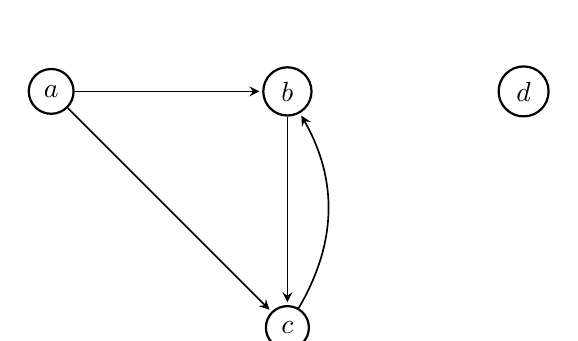
\begin{tikzpicture}[
            > = stealth, % arrow head style
            shorten > = 1pt, % don't touch arrow head to node
            auto,
            node distance = 3cm, % distance between nodes
            semithick % line style
        ]

        \tikzstyle{every state}=[
            draw = black,
            thick,
            fill = white,
            minimum size = 4mm
        ]

        \node[state] (a) {$a$};
        \node[state] (b) [right of=a] {$b$};
        \node[state] (c) [below of=b] {$c$};
	\node[state] (d) [right of=b] {$d$};
       
	\path[->] (a) edge (b);
	\path[->] (a) edge (c);
	\path[->] (b) edge (c);
	\path[->] (c) [bend right] edge (b);
	%\path[->] (1)  [loop above] edge (1);
	

        %\draw[red, dashed] (1, 2) -- (1, -2);
    \end{tikzpicture}
$$

draw the directed graph of

(a) The reflexive closure of the relation.

(b) The symmetric closure of the relation.

(c) The transitive closure of the relation.

\subsection{Solution}

\textbf{(a) reflexive closure:}

$$
  \begin{tikzpicture}[
            > = stealth, % arrow head style
            shorten > = 1pt, % don't touch arrow head to node
            auto,
            node distance = 3cm, % distance between nodes
            semithick % line style
        ]

        \tikzstyle{every state}=[
            draw = black,
            thick,
            fill = white,
            minimum size = 4mm
        ]

        \node[state] (a) {$a$};
        \node[state] (b) [right of=a] {$b$};
        \node[state] (c) [below of=b] {$c$};
	\node[state] (d) [right of=b] {$d$};
       
	\path[->] (a) edge (b);
	\path[->] (a) edge (c);
	\path[->] (b) edge (c);
	\path[->] (c) [bend right] edge (b);

	\path[->] (a)  [loop left] edge (a);
	\path[->] (b)  [loop above] edge (b);
	\path[->] (c)  [loop below] edge (c);
	\path[->] (d)  [loop right] edge (d);
    \end{tikzpicture}
$$

\textbf{(b) symmetric closure:}

$$
  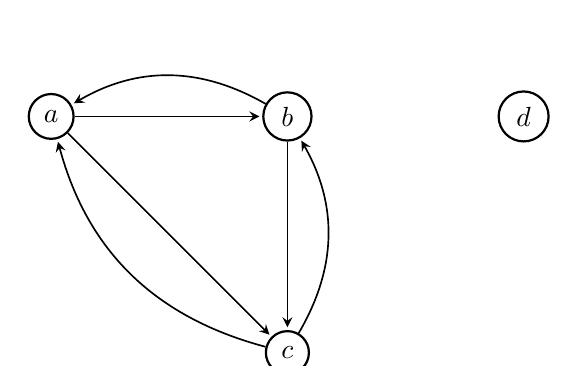
\begin{tikzpicture}[
            > = stealth, % arrow head style
            shorten > = 1pt, % don't touch arrow head to node
            auto,
            node distance = 3cm, % distance between nodes
            semithick % line style
        ]

        \tikzstyle{every state}=[
            draw = black,
            thick,
            fill = white,
            minimum size = 4mm
        ]

        \node[state] (a) {$a$};
        \node[state] (b) [right of=a] {$b$};
        \node[state] (c) [below of=b] {$c$};
	\node[state] (d) [right of=b] {$d$};
       
	\path[->] (a) edge (b);
	\path[->] (a) edge (c);
	\path[->] (b) edge (c);
	\path[->] (c) [bend right] edge (b);

	\path[->] (b) edge [bend right] (a);
	\path[->] (c) edge [bend left] (a);
    \end{tikzpicture}
$$

\textbf{(c) transitive closure:}

$$
  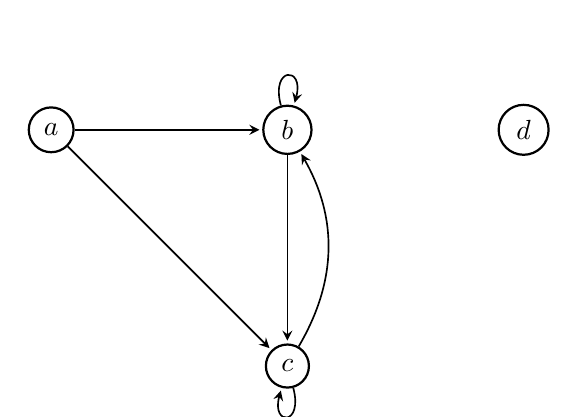
\begin{tikzpicture}[
            > = stealth, % arrow head style
            shorten > = 1pt, % don't touch arrow head to node
            auto,
            node distance = 3cm, % distance between nodes
            semithick % line style
        ]

        \tikzstyle{every state}=[
            draw = black,
            thick,
            fill = white,
            minimum size = 4mm
        ]

        \node[state] (a) {$a$};
        \node[state] (b) [right of=a] {$b$};
        \node[state] (c) [below of=b] {$c$};
	\node[state] (d) [right of=b] {$d$};
       
	\path[->] (a) edge (b);
	\path[->] (a) edge (c);
	\path[->] (b) edge (c);
	\path[->] (c) [bend right] edge (b);

	\path[->] (b)  [loop above] edge (b);
	\path[->] (c)  [loop below] edge (c);
    \end{tikzpicture}
$$

%----------------------------------------------------------------------------------------
%	PROBLEM 5
%----------------------------------------------------------------------------------------

\section{Exercise}

Let R be represented by the matrix

$$M_R = \begin{bmatrix}
0 & 0 & 0  \\
1 & 0 & 1  \\
1 & 1 & 0 \\
\end{bmatrix}$$

(a) Give the matrix that represents the reflexive closure of R, r(R):

(b) Give the matrix that represents the symmetric closure of R, s(R):

\subsection{Solution}

\textbf{(a) reflexive closure:}

$$M_{r(R)} = \begin{bmatrix}
1 & 0 & 0  \\
1 & 1 & 1  \\
1 & 1 & 1 \\
\end{bmatrix}$$

\textbf{(b) symmetric closure:}

$$M_{s(R)} = M_R \cup M_{R^{-1}} = \begin{bmatrix}
0 & 0 & 0  \\
1 & 0 & 1  \\
1 & 1 & 0 \\
\end{bmatrix} \cup 
\begin{bmatrix}
0 & 1 & 1  \\
0 & 0 & 1  \\
0 & 1 & 0 \\
\end{bmatrix} = 
\begin{bmatrix}
0 & 1 & 1  \\
1 & 0 & 1  \\
1 & 1 & 0 \\
\end{bmatrix}$$

%----------------------------------------------------------------------------------------
%	PROBLEM 6
%----------------------------------------------------------------------------------------

\section{Exercise}

Prove directly that if the relation $R$ is symmetric, then its transitive closure, $t(R) = R^*$, is also symmetric.

\subsection{Solution}

Let $R$ be a symmetic relation on the set $S$, let $t(R)$ be the transitive closure of $R$, and let $(a,b) \in t(R)$. By the definition of a transitive closure $\exists n \in \mathbb{N}$ such that $(a, b) \in R^n$. Therefor there must have been some chain in R that produced this, thus there was some $x_0, x_1,..., x_n$ such that:

$$x_0 = a$$
$$x_n = b$$
For $k = 0,..., n - 1 \vert (x_k, x_{k+1}) \in R$

Now we can essentially reverse each relation in this chain from the fact that R is symmetric, or:

For $k = 0,...,n$ let $y_k = x_{n-k}$

Then:

$$y_0 = x_n = b$$
$$y_n = x_0 = a$$

For $k = 0,...,n -1\vert (x_{n-k-1}, x_{n-k}) \in R$ thus $(y_{k+1}, y_k) \in R$

Since R is symmetric, for $k = 0,...,n-1 \vert (y_k, y_{k+1}) \in R$ thus $(b,a) \in R^n$ and $(b,a) \in t(R)$ therefore the transitive closure is also symmetric.


%----------------------------------------------------------------------------------------
%	END DOCUMENT
%----------------------------------------------------------------------------------------

\end{document}